% !TeX root = ../main.tex

\chapter{多级双重推理网络}\label{cha:HDRNet}
本章将介绍多级双重推理网络(Hierarchical Dual Reasoning Network, HDR Net)。顾名思义,HDR Net能够在多个分辨率等级上执行步骤内和步骤间的推理。HDR Net由两个重要模块构成,即步骤内推理模块(Intra-step Reasoning Module)和步骤间推理模块(Cross-step Reasoning Module)。在第~\ref{sec:ISR}~节和第~\ref{sec:CSR}~节中,本文将分别介绍步骤内推理模块和步骤间推理模块,最后在第~\ref{sec:whole}~节中介绍网络的整体结构。
\section{步骤内推理模块}\label{sec:ISR}
步骤内推理模块的作用是在每个步骤内的不同帧之间完成时序的推理,该模块使用一个双向RNN实现,如图~\ref{fig:birnn}~所示,图中展示了输入序列长度为4时的情况,对于步骤内推理模块,该长度应该是每个步骤中的帧数。
\begin{figure}[htbp]
    \centering
    \includegraphics[width=\textwidth,page=2]{hdrnet.pdf}
    \caption{双向RNN示意图}
    \label{fig:birnn}
\end{figure}
使用双向RNN来实现推理模块是基于以下几个原因:
\begin{enumerate}
    \item RNN是为了对序列建模而设计的,所以自然适合于时序上的推理;
    \item RNN的输入序列长度可以变化,可以适应不同步骤数目的情况;
    \item 双向RNN保证了每一步的推理都能够考虑到前面的步骤和后面的步骤。
\end{enumerate}

在步骤内不理模块中,RNN的输入序列为:
\begin{equation}
    \prescript{\intra}{}{S}^{(k)}_i = \left[f^{(k)}_{i, 1}, f^{(k)}_{i, 2}, \ldots, f^{(k)}_{i, n}\right].
\end{equation}
上式中$k$表示第$k$个分辨率,$n$表示每个步骤内的帧数,则$f^{(k)}_{i, j}$表示第$i$个步骤中第$j$帧的第$k$级特征。由此可见,在同一个分辨率,所有的步骤共享一个步骤内推理模块。双向RNN的两个方向的输出直接取平均作为最终的输出,记作$\prescript{\intra}{}{R}^{(k)}_i$,即
\begin{equation}
    \prescript{\intra}{}{R}^{(k)}_i = \birnn\left(\prescript{\intra}{}{S}^{(k)}_i\right).
\end{equation}
在标准的RNN实现中,每个RNN单元中都是使用全连接层实现映射,并不适用于对不同分辨率的视觉特征。所以,HDR Net中使用的RNN单元是本文自定义的,如图~\ref{fig:rnn_cell}~所示,图中汇聚的箭头表示相加运算,分支的箭头表示运算结果的复用。
\begin{figure}[htbp]
    \centering
    \includegraphics[width=\textwidth,page=3]{hdrnet.pdf}
    \caption{HDR Net 中的RNN单元}
    \label{fig:rnn_cell}
\end{figure}

每个RNN单元中的定义如下:
\begin{equation}
    \begin{split}    
    &\vh_{j} = \relu(\norm(\conv(\vx_{j}))) + \relu(\norm(\conv(\vh_{j-1}))),\\
        &\vy_j = \relu(\norm(\conv(\vh_j))).
    \end{split}
\end{equation}
上式中$j$为RNN单元的序号,$\vh_{0}$表示初始的因变量,本文中将其初始化为全零值。每个卷积层的卷积核大小都是$1\times 1$,且输入输出通道数目相同。这样定义的RNN单元可以很好地应用在视觉特征上,同时又可以极大地减小计算量。实验发现,由于视频溯因推理任务中每个问题中包括大量图片,在训练的过程中如果使用batch normalization(批归一化)则会因为batch size太小导致统计量不准确,训练不稳定,所以在实验中用group normalization (组归一化)来完成归一化操作。

由步骤内推理模块的定义可知,所有的特征的尺寸经过该模块之后不会发生改变,这就方便了之后使用残差连接的方式来更新特征。

\section{步骤间推理模块}\label{sec:CSR}
步骤间推理模块的作用是对不同步骤以及两个观测的信息进行推理。但是由于每个步骤中有$n$帧图片,而每个观测中只有一个图片,无法将它们的特征构成一个序列。所以,我们首先利用步骤内推理模块的输出$\prescript{\intra}{}{R}^{(k)}_i$,在时间上取平均,得到了每一步骤的特征$p_i^{(k)}$:
\begin{equation}
    p_i^{(k)} = \frac{1}{n}\sum_{j=1}^n\prescript{\intra}{}{R}^{(k)}_{i,j}.
\end{equation}
上式中$\prescript{\intra}{}{R}^{(k)}_{i,j}$表示在第$k$个分辨率上,第$i$个步骤的第$j$帧的步骤内推理模块的输出。将两个观测$O_1,O_2$在第$k$个分辨率的特征记作$o_1^{(k)}$和$o_2^{(k)}$,此时$o_1^{(k)}$和$o_2^{(k)}$与$p_i^{(k)}$具有相同的维度,将它们按照时间顺序排列,即可得到步骤间推理模块的输入序列:
\begin{equation}
    \prescript{\cross}{}{S}^{(k)} = [o_1^{(k)}, p_1^{(k)}, p_2^{(k)}, \ldots, p_l^{(k)}, o_2^{(k)}].
\end{equation}
上式中$l$表示步骤数目。可见为了更好地表示时序关系,输入序列中特征排列顺序与事件发生的先后顺序一致。与步骤内推理模块一样,步骤间推理模块也采用双向RNN实现,其结构如图~\ref{fig:birnn}~和图~\ref{fig:rnn_cell}~所示。设RNN的输出为$\prescript{\cross}{}{R}^{(k)}$,则
\begin{equation}
    \prescript{\cross}{}{R}^{(k)} = \birnn\left(\prescript{\cross}{}{S}^{(k)}\right).
\end{equation}
考虑到$\prescript{\cross}{}{R}^{(k)}$中同时包含两个观测和所有步骤的输出,可以写成:
\begin{equation}
    \prescript{\cross}{}{R}^{(k)} = \left[\prescript{\cross}{\rm o}{R}_1^{(k)},\prescript{\cross}{\rm h}{R}_1^{(k)},\prescript{\cross}{\rm h}{R}_2^{(k)}\ldots, \prescript{\cross}{\rm h}{R}_l^{(k)},\prescript{\cross}{\rm o}{R}_2^{(k)}\right].
\end{equation}
其中下角标$\mathrm{o}$表示观测(observation),下角标$\mathrm{h}$表示假设(hypothesis)。最后,我们将步骤间推理模块和步骤内推理模块的输出结果通过残差连接\cite{he2016deep}的方式用来更新所有的特征:
\begin{equation}
    \begin{aligned}
        &f_{i, j}^{(k)}\leftarrow f_{i, j}^{(k)} + \prescript{\intra}{}{R}_{i, j}^{(k)}  +\prescript{\cross}{\rm h}{R}_i^{(k)}, &(1\le i \le l)\\
        &o_{i}^{(k)} \leftarrow o_{i}^{(k)} + \prescript{\cross}{\rm o}{R}_i^{(k)}. &(i = 1, 2)
    \end{aligned}
\end{equation}
残差连接的方式可以使训练的过程更加稳定,尤其是对于比较深的主干网络。另外,在训练初期,使用残差连接的方式可以充分利用经典的2D卷积网络在空间上提取特征的能力,并通过时序推理的方法逐步优化特征。

综上所述,步骤内推理模块和步骤间推理模块相互配合,共同完成了两个层次的推理。在实际使用中,它们也总是以串联的方式出现,所以可以将它们统称为多级双重推理模块(HDR Module)。图~\ref{fig:HDR_Module}~是HDR Module 的一个示意图,图中展示了在$n=4,l=3$的情况下上文所述的运算过程。
\begin{figure}[htbp]
    \centering
    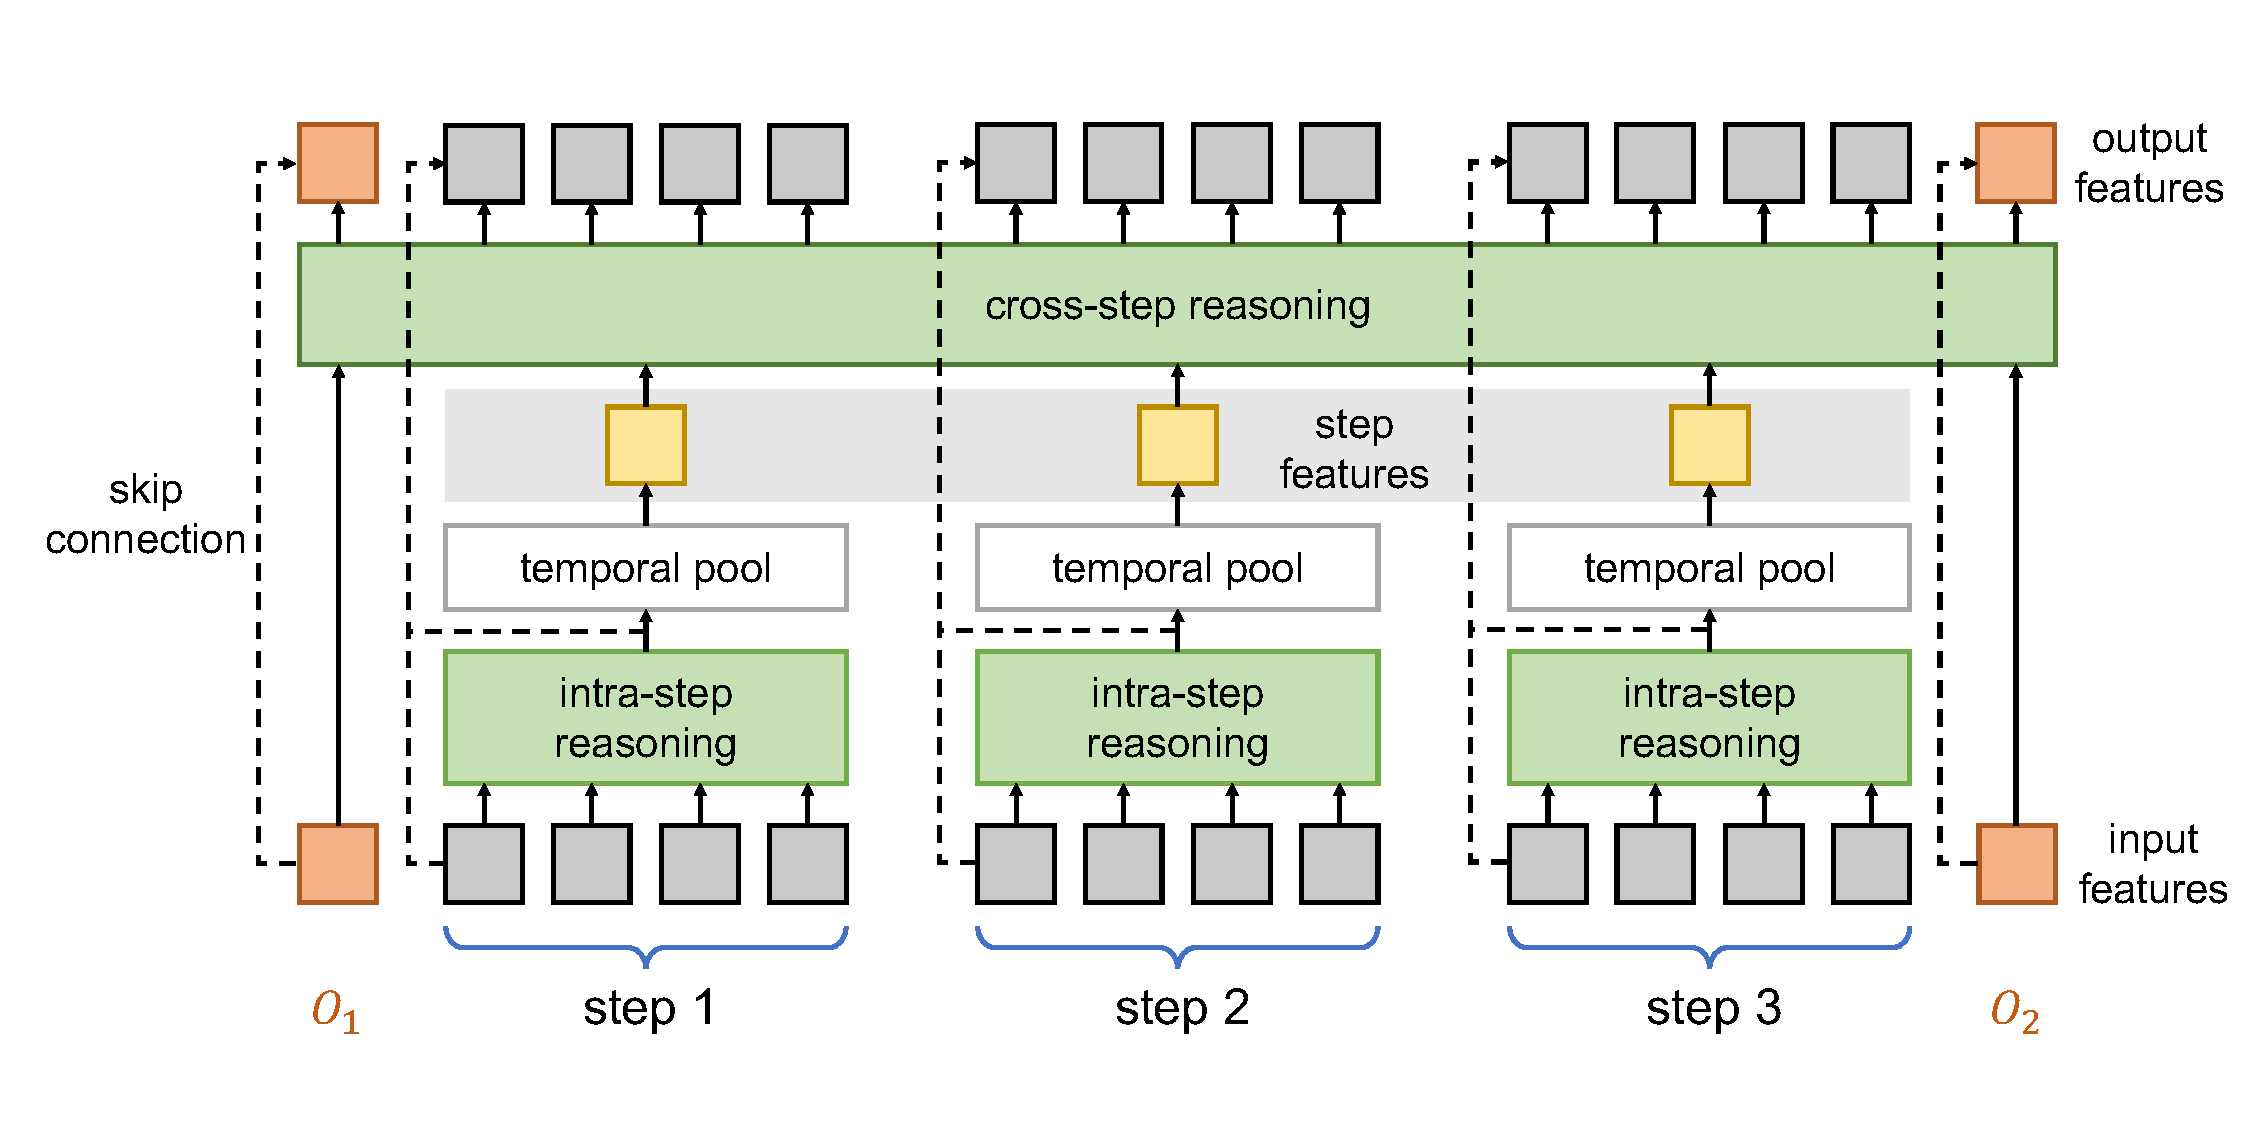
\includegraphics[width=\textwidth,page=1]{hdrnet.pdf}
    \caption{多级双重推理模块}
    \label{fig:HDR_Module}
\end{figure}
\section{网络整体结构}\label{sec:whole}
本节将介绍如何利用多级双重推理模块来构建网络,即HDR Net的整体结构。为了充分利用2D卷积网络对空间信息提取的能力,HDR Net的主干网络使用ResNet18\cite{he2016deep}来实现,并在每个空间上的池化层后面增加一个HDR Module。

\begin{figure}[htbp]
    \centering
    \includegraphics[page=4,,trim=0cm 4cm 0cm 4cm,clip,width=\textwidth]{hdrnet.pdf}
    \caption{HDR Net网络整体结构}
    \label{fig:hdrnet}
\end{figure}
图~\ref{fig:hdrnet}~中绿色的部分是本文提出的HDR Module(如图~\ref{fig:HDR_Module}~),其他部分则与ResNet18相同。由于HDR Module已经在时间维度占用了较多的计算量,为了减少计算量,使用了如下几个方法:
\begin{enumerate}
    \item 使用层数较少的主干网络,即ResNet18而不是更深的网络;
    \item 在标准的ResNet18的基础上,将所有通道数目减半;
    \item 在第一个HDR Module 后面紧接着一个时间维度的池化层,该操作将每个步骤中的8帧减少为每个步骤4帧。
\end{enumerate}

最后一个HDR Module 后面的池化层同时对时间和空间上取平均,得到了最终的时间和空间上的特征。在VideoABC数据集中,每个问题中都有四个选项,HDR Net会将每个选项分别处理,最后的全连接网络将池化层输出的特征映射到一个实数,作为每个选项的得分,也就是说,最终预测的选项为:

\begin{equation}
    H^* = \argmax_{H_i} \HDRNet\left(O_1, O_2, H_i\right)
\end{equation}
在训练时,使用交叉熵损失函数:
\begin{equation}
    \gL = -\log\frac{\exp{\HDRNet(O_1, O_2, H_+)}}{\displaystyle\sum_{i=1}^4\exp{\HDRNet(O_1, O_2, H_i)}}
\end{equation}

